%%%%%%%%%%%%%%%%%%%%%%%%%%%%%%%%%%%%%%%%%%%%%%%%%%%%%%%%%%%%%%%%%%%%%%%%%%
\chapter{Étude de Projet}
\label{Chapitre1}
\addtocontents{mtc}{\protect\renewcommand{\protect\insertminitoc}{}}
%%%%%%%%%%%%%%%%%%%%%%%%%%%%%%%%%%%%%%%%%%%%%%%%%%%%%%%%%%%%%%%%%%%%%%%%%%
\section{Introduction}
\label{sec:Introduction1}
%%%%%%%%%%%%%%%%%%%%%%%%%%%%%%%%%%%%%%%%%%%%%%%%%%%%%%%%%%%%%%%%%%%%%%%%%%

 Dans le cadre de la réussite d’un projet, la réalisation d’une analyse préliminaire approfondie s’avère indispensable. Cette étape permet d’étudier les différentes dimensions du projet et d’en apprécier les impacts potentiels. Elle vise également à établir un cadre de référence en mettant en évidence les atouts et les limites des solutions existantes, tout en identifiant des axes d’amélioration pertinents. À cet effet, nous entamerons cette étude par une présentation générale du projet, suivie d’une analyse critique de l’existant et de la solution proposée. Enfin, nous exposerons les méthodologies adoptées ainsi que les technologies et outils mis en œuvre.
%%%%%%%%%%%%%%%%%%%%%%%%%%%%%%%%%%%%%%%%%%%%%%%%%%%%%%%%%%%%%%%%%%%%%%%%%%
\section{Présentation de l'Organisme d'Accueil}
\label{sec:organisme}
%%%%%%%%%%%%%%%%%%%%%%%%%%%%%%%%%%%%%%%%%%%%%%%%%%%%%%%%%%%%%%%%%%%%%%%%%%

\textit{"\textbf{Yes Internet} est une société tunisienne spécialisée dans le développement de solutions numériques et de services informatiques. Elle aide ses clients à transformer numériquement leurs activités en leur proposant des applications web sur mesure, des solutions de gestion ainsi que des services d'hébergement.''}\cite{yesinternet}

\begin{figure}[H]
    \centering
    
\includegraphics[width=0.2\textwidth]{Chapitres/Figures/Yesinternet.png}
    \caption{Logo de Yes Internet}
    \label{fig:logo_yes}
\end{figure}
\textbf{Yes Internet} propose une gamme de services adaptés aux besoins des entreprises 
tunisiennes, notamment :
\begin{itemize}
    \item Création d'applications web et mobiles sur mesure
    \item Conseil et accompagnement en matière digitale
    \item Services d'hébergement et de maintenance informatique
    \item Intégration de solutions de gestion métier
\end{itemize}

%%%%%%%%%%%%%%%%%%%%%%%%%%%%%%%%%%%%%%%%%%%%%%%%%%%%%%%%%%%%%%%%%%%%%%%%%%
\subsection{Structure organisationnelle}
%%%%%%%%%%%%%%%%%%%%%%%%%%%%%%%%%%%%%%%%%%%%%%%%%%%%%%%%%%%%%%%%%%%%%%%%%%
La Figure \ref{fig:organigramme} présente l'organigramme de la société Yes Internet.
 
\begin{figure}[H]
    \centering
    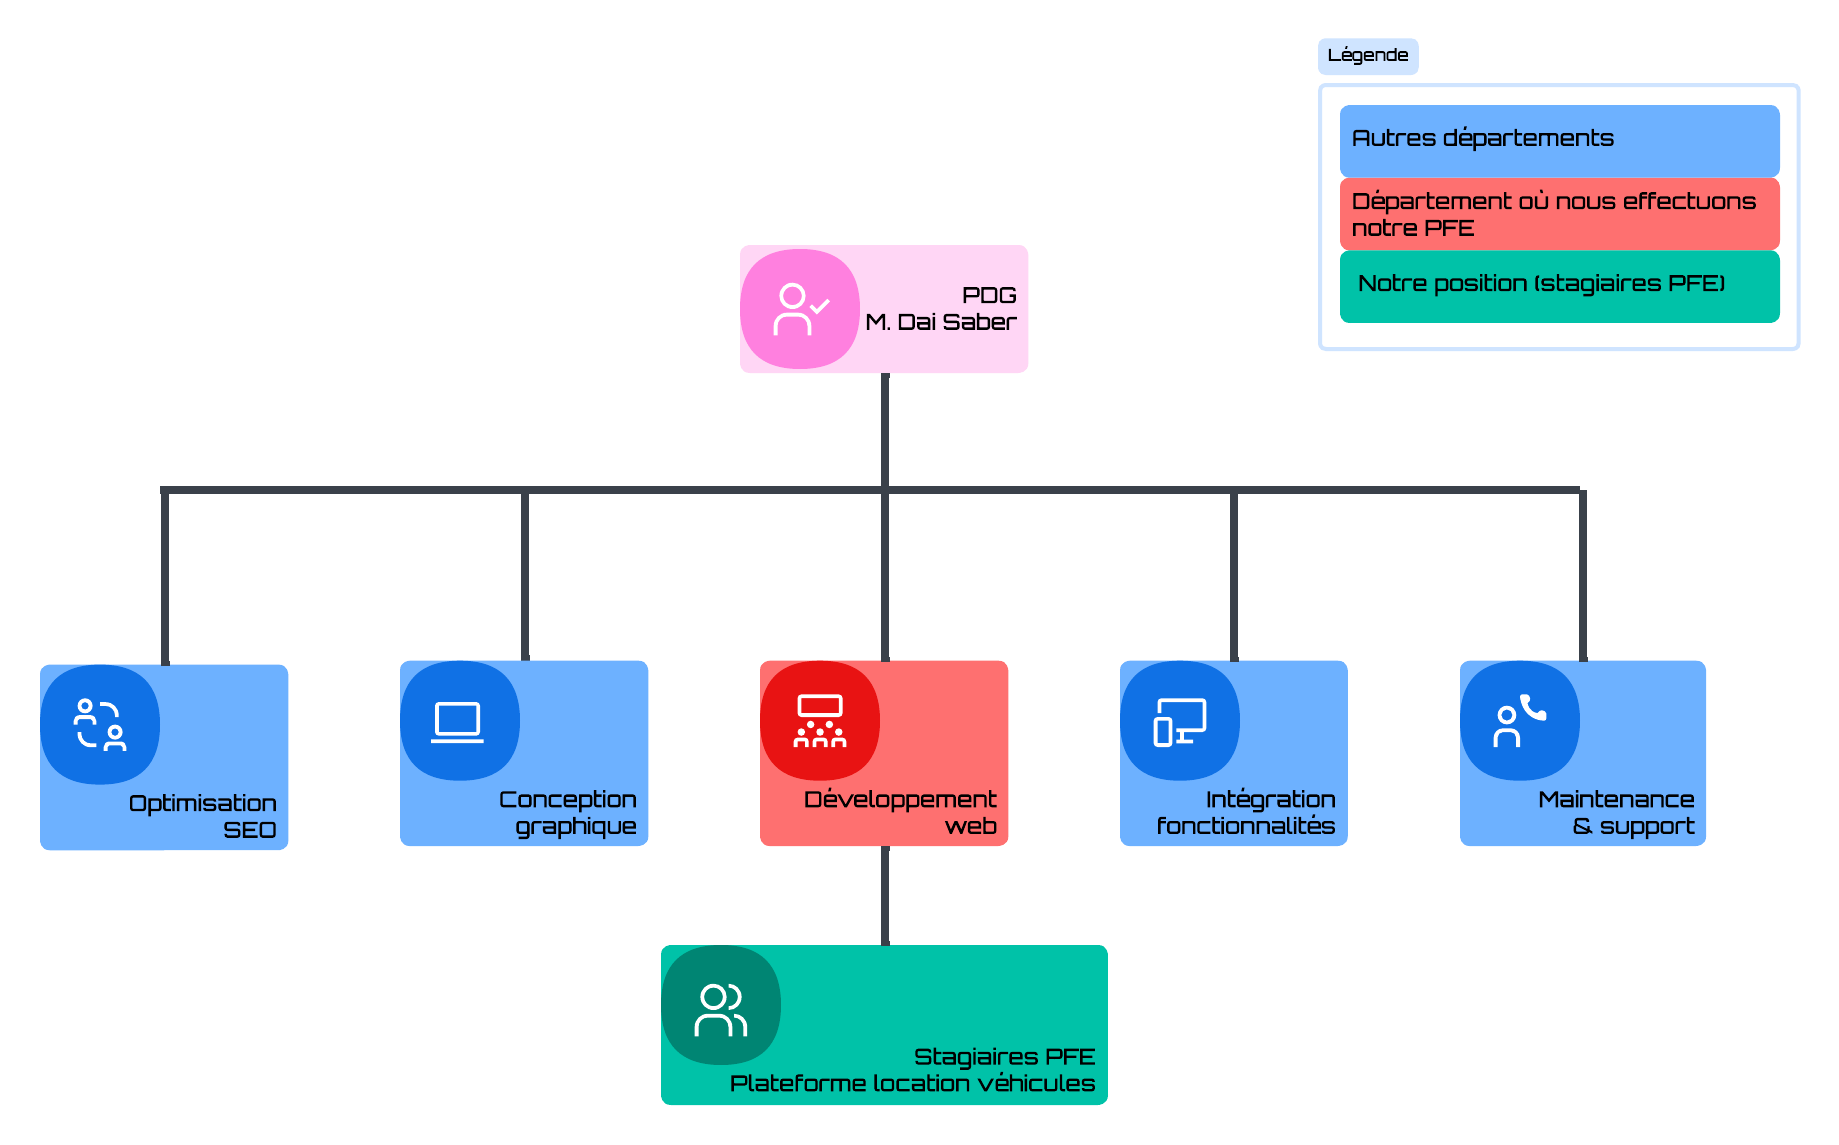
\includegraphics[width=1\textwidth]{Chapitres/Figures/organigramme.png}
    \caption{Organigramme de Yes Internet}
    \label{fig:organigramme}
\end{figure}

Dans le cadre de notre projet de fin d'études, nous sommes intégrés au sein du \textbf{départ-\\ement Développement Web}, sous la supervision directe du responsable 
technique. Notre mission consiste à concevoir et développer la plateforme intelligente 
de gestion de location de véhicules multi-agences.

%%%%%%%%%%%%%%%%%%%%%%%%%%%%%%%%%%%%%%%%%%%%%%%%%%%%%%%%%%%%%%%%%%%%%%%%%%
\section{Cadre et Présentation du Projet}
\label{sec:presentation}
%%%%%%%%%%%%%%%%%%%%%%%%%%%%%%%%%%%%%%%%%%%%%%%%%%%%%%%%%%%%%%%%%%%%%%%%
Dans le cadre de notre projet de fin d’études, l’entreprise \textbf{Yes Internet} nous a confié la réalisation d’un projet intitulé \textit{ Plateforme Intelligente de Gestion de Location de Véhicules Multi-Agences }. Ce projet constitue une opportunité de mobiliser et de mettre en application l’ensemble des connaissances théoriques et des compétences pratiques acquises tout au long de notre formation à l’École Supérieure d’Économie Numérique. Il s’inscrit également dans la perspective de l’obtention du diplôme de licence en informatique de gestion.
%%%%%%%%%%%%%%%%%%%%%%%%%%%%%%%%%%%%%%%%%%%%%%%%%%%%%%%%%%%%%%%%%%%%%%%%%%
\newpage
\section{Analyse de l'Existant}
\label{sec:existant}
%%%%%%%%%%%%%%%%%%%%%%%%%%%%%%%%%%%%%%%%%%%%%%%%%%%%%%%%%%%%%%%%%%%%%%%%%%
L'analyse de l'existant vise à enrichir l'étude des pistes innovantes 
d'un projet en cours de conception, avant sa mise en œuvre. Cette étude 
préalable permet de se faire une idée de la pertinence du projet, de sa 
faisabilité et de sa continuité.\cite{etude_faisabilite_cairn} 

\medskip

D'après notre analyse, le secteur de la gestion et suivie de location de véhicules dispose de plusieurs solutions à l'échelle internationale, mais les agences locales tunisiennes restent largement sous-équipées sur le plan numérique. Il devient donc crucial de réaliser une évaluation approfondie des systèmes actuels tant au niveau national qu'international.

%%%%%%%%%%%%%%%%%%%%%%%%%%%%%%%%%%%%%%%%%%%%%%%%%%%%%%%%%%%%%%%%%%%%%%%%%%
\subsection{Étude des solutions existantes au niveau national}
%%%%%%%%%%%%%%%%%%%%%%%%%%%%%%%%%%%%%%%%%%%%%%%%%%%%%%%%%%%%%%%%%%%%%%%%%%
Après avoir effectué des recherches liées aux applications numériques utilisées pour gérer le processus de location de véhicules en Tunisie, nous avons constaté que les pratiques adoptées par les agences locales varient en fonction des moyens et des outils disponibles.

Selon certaines études, le secteur de la location de voitures en Tunisie compte plusieurs centaines d’agences, ce qui témoigne de l’importance de cette activité et de la diversité des modes de gestion adoptés \cite{letemps_news}.

\begin{itemize}[noitemsep, topsep=0pt]
    \item \textbf{Processus de location et de réservation en Tunisie  :} \\Le client se rend directement à l’agence pour louer un véhicule. L’agent collecte les informations nécessaires, telles que les coordonnées du client, le type de véhicule souhaité, la durée de location et les documents requis (permis de conduire, carte d’identité, etc.). Le contrat de location est ensuite établi à partir de modèles standards utilisés dans le domaine \cite{scribd_contrat_standard}. Les informations relatives à la réservation, au contrat et à la disponibilité des véhicules sont consignées dans des supports internes tels que des registres ou des fichiers de suivi.


    \item \textbf{Suivi opérationnel et gestion de flotte :} \\Les agences utilisent des fiches de suivi ou des supports de pointage pour enregistrer les mouvements des véhicules (mise à disposition, retour, état du véhicule).


    \item \textbf{Contrats et gestion financière :} \\Les contrats de location, les paiements, les factures et les cautions sont enregistrés à l’aide des supports manuelles, fin de constituer un historique des opérations effectuées.  
     \\Exemple ci‑dessous :
    \\ \textit{Contrats de location papier} : Les agences utilisent fréquemment des formulaires papier pré-imprimés pour établir les contrats de location, nécessitant une saisie manuelle des informations client et véhicule, puis ces contrats sont archivés sous forme papier, servant à établir un historique des opérations de l’agence. 
        \\(Voir Figure \cite{modele-contrat-location-vehicule}).




    \item \textbf{Utilisation d’outils informatiques standards :}\\ Certaines agences s’appuient sur des outils tels que des tableurs pour organiser les réservations et suivre les informations liées aux clients et aux véhicules \cite{youtube_excel_gestion}.
    Exemple ci‑dessous :
    \\ \textit{Gestion de flotte via Excel} : Certaines agences utilisent des feuilles de calcul Excel pour gérer leur flotte, les réservations et la facturation, ce qui est sujet aux erreurs et manque d'automatisation. (Voir Figure \cite{gestion-de-location-par_excel}).
\end{itemize}
%%%%%%%%%%%%
\begin{figure}[H]
    \centering
    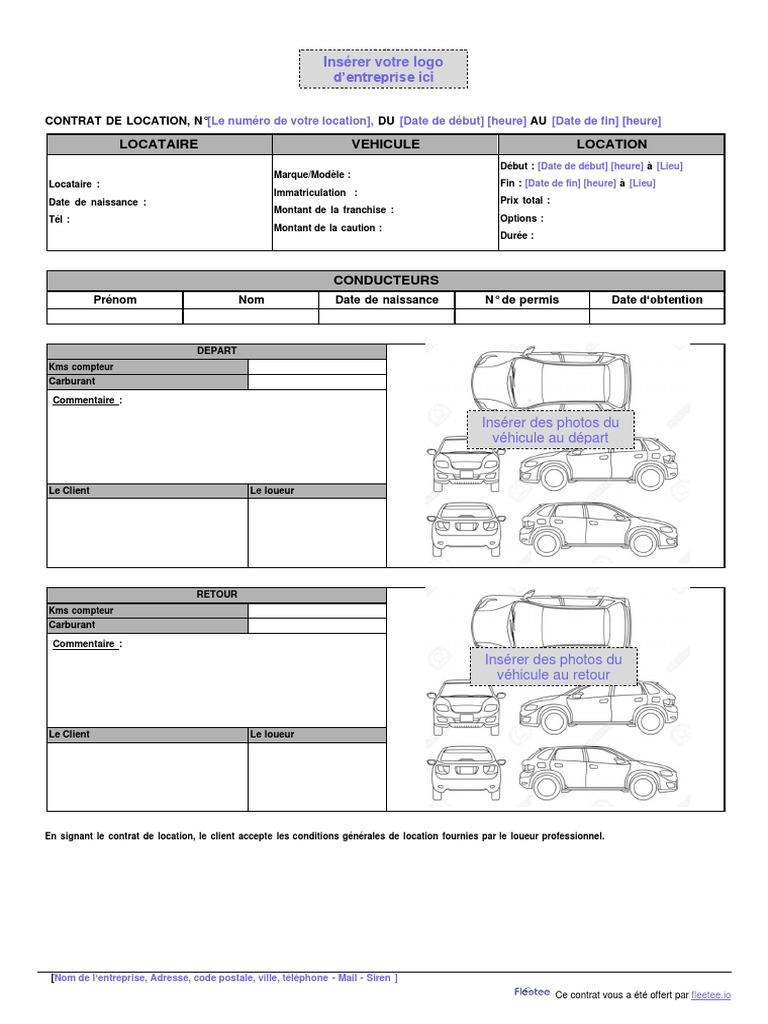
\includegraphics[width=0.8\textwidth]{Chapitres/Figures/contrat_papier.jpg}
    \caption{Modèle de contrat de location de véhicule. \cite{modele-contrat-location-vehicule} }
    \label{fig:contrat}
\end{figure}
%%%%%%%%%%%%
\begin{figure}[H]
    \centering
    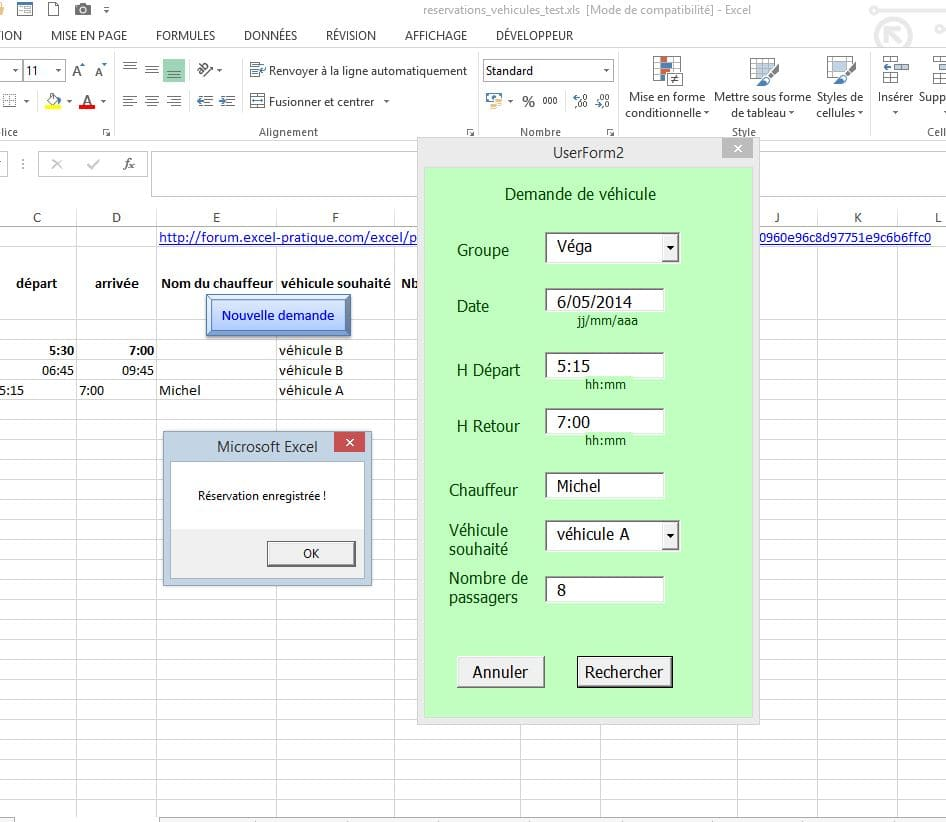
\includegraphics[width=1\textwidth]{Chapitres/Figures/gestion_excel.jpg}
    \caption{Gestion de locations des voitures par Excel.\cite{gestion-de-location-par_excel}}
    \label{fig:excel}
\end{figure}

\begin{itemize}[noitemsep, topsep=0pt]
    \item \textbf{Solutions numériques spécialisées pour la location :}\\
En parallèle, il existe des solutions numériques dédiées à la gestion de la location de véhicules. \textbf{Des logiciels spécialisés} proposent des fonctionnalités telles que la gestion des réservations, le suivi de la flotte automobile et la facturation \cite{renthub_tarifs}\cite{Logiciel_de_gestion_des_locations}. De même, certaines \textbf{plateformes en ligne} permettent de consulter les offres de location et d’effectuer des réservations à distance \cite{tunisiadrive_benefits}.
\end{itemize}
%%%%%%%%%%%%
\begin{figure}[H]
    \centering
    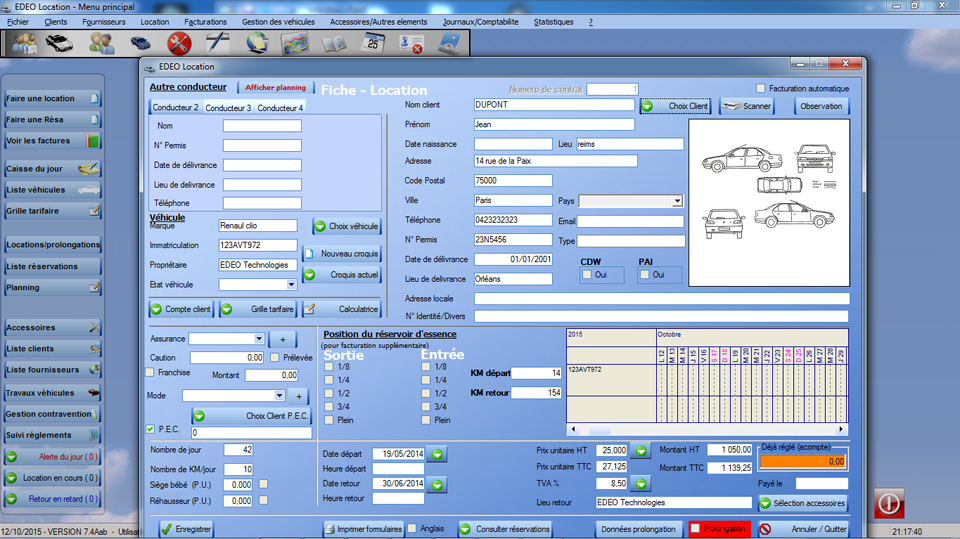
\includegraphics[width=0.9\textwidth]
    {Chapitres/Figures/exmp_sys.png}
    \caption{EDEO: Logiciel interne de gestion des locations.\cite{Logiciel_de_gestion_des_locations} }
    \label{fig:exmp_sys}
\end{figure}
%%%%%%%%%%%%%
\begin{figure}[H]
    \centering
    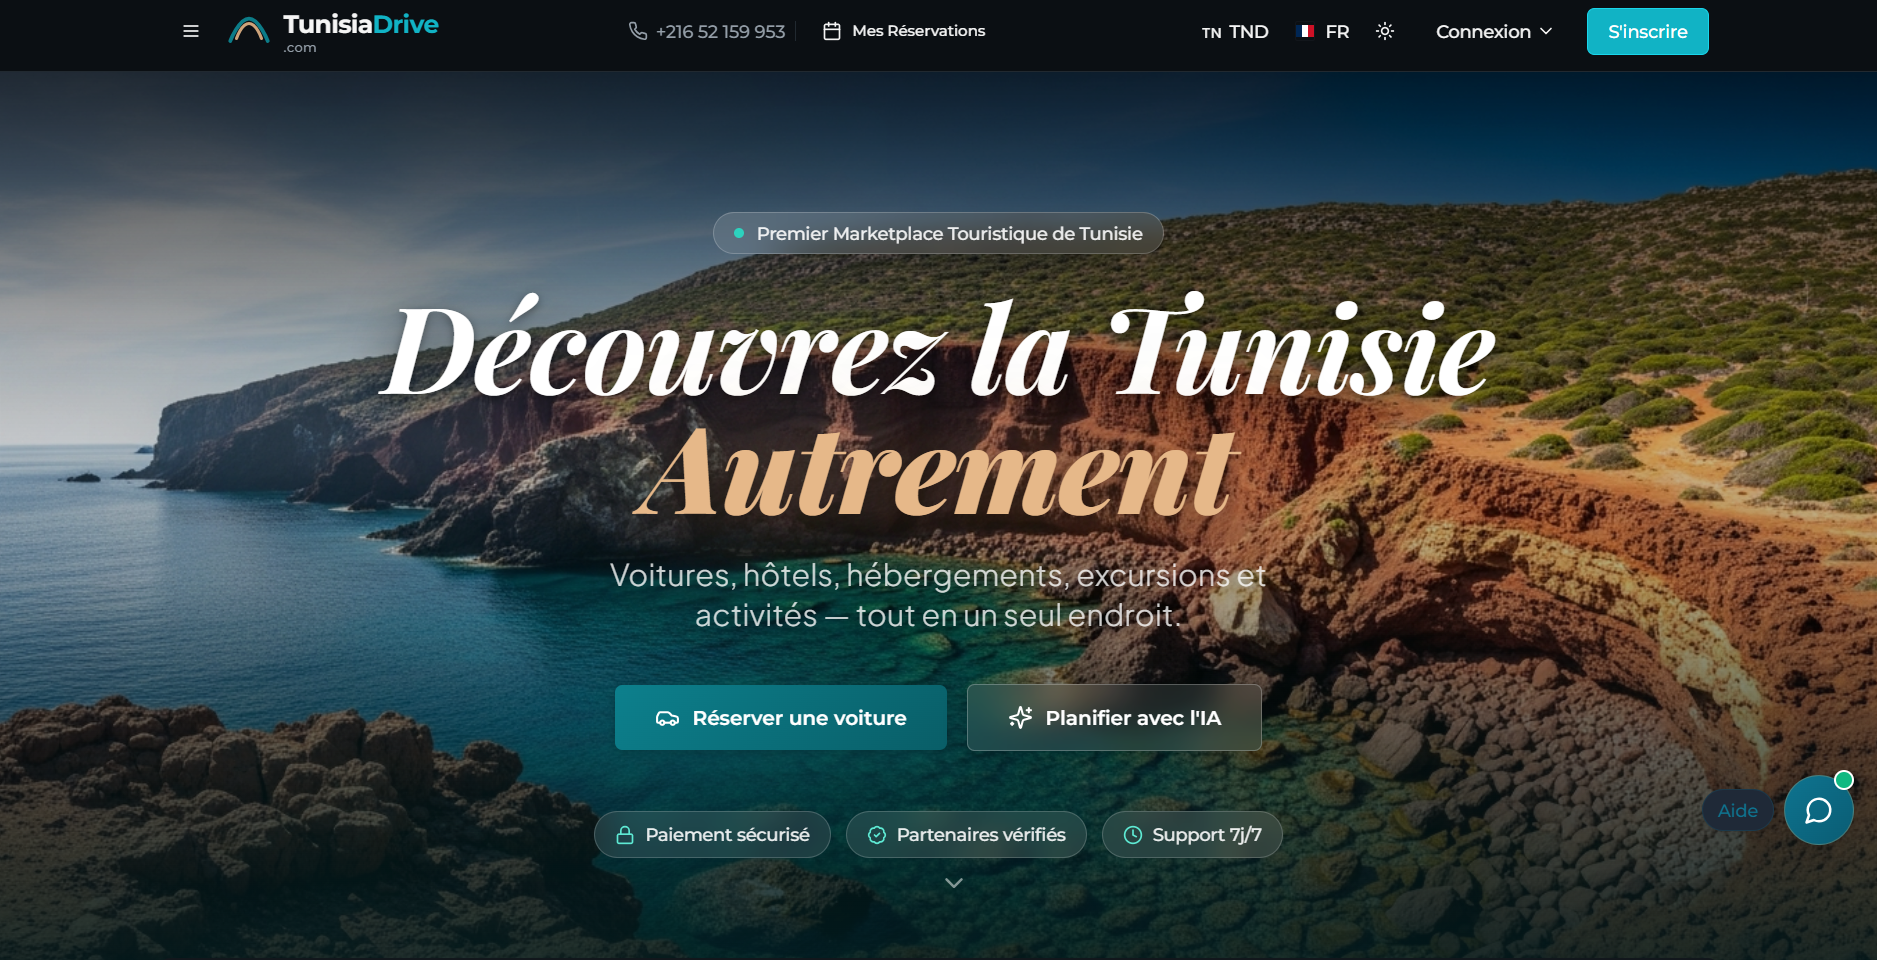
\includegraphics[width=0.9\textwidth]
    {Chapitres/Figures/tunisiadr.png}
    \caption{Plateforme de locations des voitures en Tunisie.\cite{tunisiadrive_benefits} }
    \label{fig:tunisiadrive}
\end{figure}
%%%%
Ainsi, ces observations montrent que les pratiques de gestion dans le domaine de la location de véhicules en Tunisie reposent sur une diversité de solutions, allant de l’utilisation de supports internes et d’outils génériques à l’intégration de solutions numériques dédiées au secteur.
%%%%

%%%%%%%%%%%%%%%%%%%%%%%%%%%%%%%%%%%%%%%%%%%%%%%%%%%%%%%%%%%%%%%%%%%%%%%%%%



\newpage
\subsection{Étude des solutions existantes au niveau international}
%%%%%%%%%%%%%%%%%%%%%%%%%%%%%%%%%%%%%%%%%%%%%%%%%%%%%%%%%%%%%%%%%%%%%%%%%%
Nous procédons ici à une analyse approfondie d'une solution de gestion de location des véhicules disponible à l'international, retenue pour sa représentativité, sa maturité et sa large adoption sur le marché mondial.
\subsubsection{Analyse de la plateforme Rent Centric}
Rent Centric est une plateforme cloud de référence dans le domaine de la gestion de location de véhicules, fondée en 2002 et utilisée par des centaines d'agences à travers le monde, notamment en Amérique du Nord, en Europe et au Moyen-Orient. Elle s'adresse aussi bien aux petites agences indépendantes qu'aux grandes entreprises multi-sites \cite{rc}.
\\La plateforme propose un ensemble de fonctionnalités permettant de couvrir l'intégralité du processus de location :
\begin{itemize}[noitemsep, topsep=0pt]
    \item \textbf{Réservation en ligne :} réservations en temps réel avec confirmation automatique et gestion des disponibilités.
    \item \textbf{Gestion de flotte :} suivi complet des véhicules, historique d'utilisation et planification de maintenance.
    \item \textbf{Gestion des contrats :} génération automatique des contrats, prolongations et gestion des retours.
    \item \textbf{Tarification dynamique :} grilles tarifaires configurables selon la saison, la durée et le profil client.
    \item \textbf{Gestion multi-agences :} administration centralisée avec tableaux de bord personnalisés par site.
    \item \textbf{Rapports et analytique :} rapports détaillés sur les performances et le taux d'occupation de la flotte.
\end{itemize}
\begin{figure}[H]
    \centering
    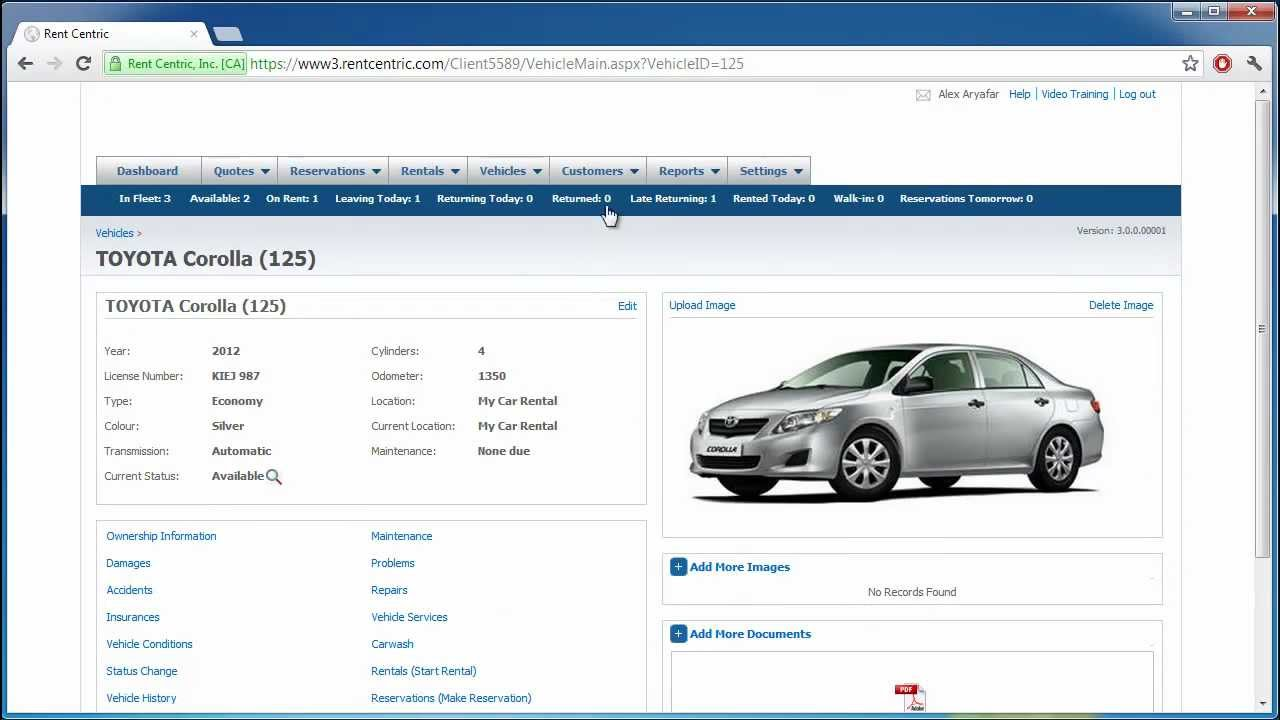
\includegraphics[width=0.85\textwidth]{Chapitres/Figures/car_centric.jpg}
    \caption{Aperçu des fonctionnalités de Rent Centric \cite{rc}}
    \label{fig:rent_centric}
\end{figure}

%%%%%%%%%%

\subsubsection{Analyse de HQ Rental Software}
HQ Rental Software est une solution complète de gestion de flotte de véhicules, conçue pour optimiser l'efficacité opérationnelle et améliorer l'expérience client. Elle offre une gamme étendue de fonctionnalités pour les entreprises de location de voitures de toutes tailles.\cite{hq_features}
\begin{itemize}[noitemsep, topsep=0pt]
    \item \textbf{Réservations et paiements en ligne :} Permet aux clients de réserver et de payer directement via un plugin de site web convivial, augmentant ainsi la portée du marché et améliorant l'expérience client.
    \item \textbf{Gestion de flotte :} Offre des outils pour gérer la disponibilité des véhicules, les réparations et les finances, réduisant la dépendance aux feuilles de calcul manuelles.
    \item \textbf{Dématérialisation :} Génère des contrats de location personnalisables qui peuvent être signés numériquement, avec la possibilité de télécharger des photos du véhicule via l'application mobile HQ.
    \item \textbf{Solutions pour divers marchés de location :} S'adapte à la location de motos, de bateaux, d'équipements et propose des solutions pour la location à long terme et le leasing.
    \item \textbf{Rapports avancés :} Fournit des tableaux de bord personnalisés pour suivre les indicateurs de performance clés et exporter les données nécessaires.
    \item \textbf{Paiements intégrés et comptabilité :} Automatise le processus de vente et la gestion des transactions financières.
    \item \textbf{Solution basée sur le cloud et accès mobile :} Accessible depuis n'importe quel appareil et n'importe où dans le monde, avec des applications Android et iOS dédiées.
\end{itemize}
\begin{figure}[H]
    \centering
    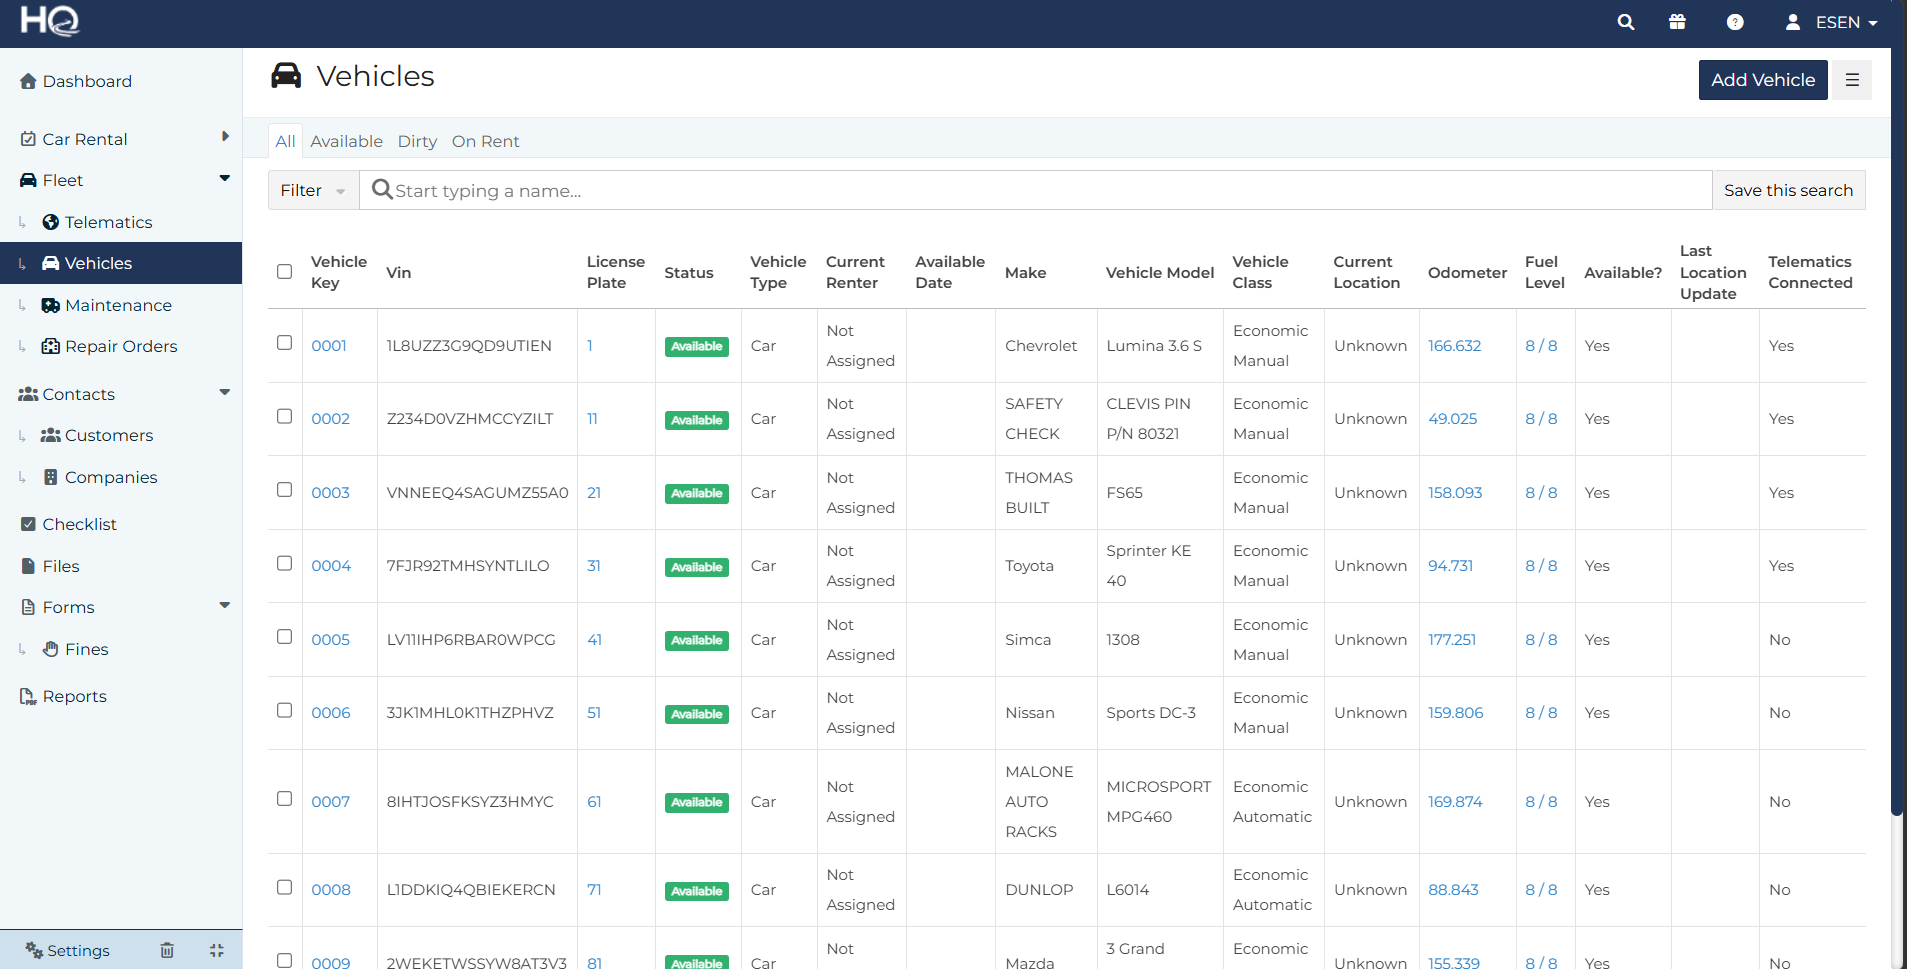
\includegraphics[width=0.85\textwidth]{Chapitres/Figures/HQ.png}
    \caption{Tableau de bord de HQ Rental Software. \cite{hq_features}}
    \label{fig:hq_dashboard}
\end{figure}

%%%%%%%%%%%%%%%%%%%%%%%%

\subsubsection{Analyse de VEVS Car Rental platform}
VEVS Car Rental Software est une solution logicielle et de site web intégrée pour les entreprises de location de voitures, visant à automatiser les processus, à rationaliser la gestion et à augmenter l'efficacité opérationnelle.\cite{vevs_features}
\begin{itemize}[noitemsep, topsep=0pt]
    \item \textbf{Réservations en ligne :} Permet aux clients de réserver des véhicules en ligne, avec des confirmations par e-mail automatiques et une page « My Booking » pour le suivi des réservations.
    \item \textbf{Gestion de flotte :} Outils pour gérer la disponibilité des véhicules, les réparations et les finances.
    \item \textbf{Tarification flexible et taxes configurables :} Permet de définir des options de tarification flexibles basées sur la durée de location et la demande, et de configurer les taxes (TVA, taxes touristiques, etc.).
    \item \textbf{Vente additionnelle d'extras et codes promotionnels :} Génère des revenus supplémentaires en proposant des extras (GPS, sièges enfant) et en créant des codes promotionnels pour les campagnes marketing.
    \item \textbf{Tarifs saisonniers et autres frais :} Permet de générer des structures de prix saisonnières distinctives et d'ajouter des frais supplémentaires (relais, jeunes conducteurs, kilométrage supplémentaire).
    \item \textbf{Solution basée sur le cloud et accès mobile :} Permet de gérer l'entreprise depuis n'importe quel appareil et n'importe où dans le monde.
\end{itemize}
\begin{figure}[H]
    \centering
    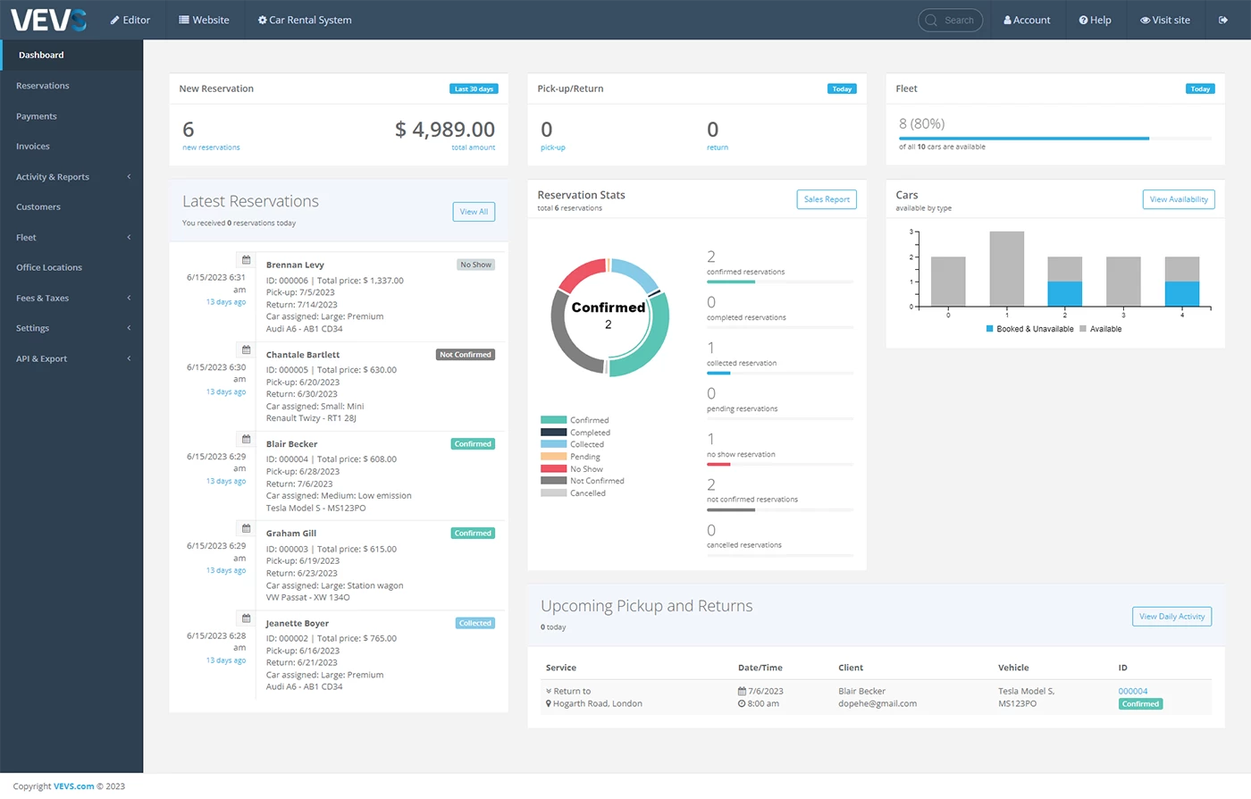
\includegraphics[width=0.8\textwidth]{Chapitres/Figures/vevs_dashboard.png}
    \caption{Tableau de bord de VEVS Car Rental platform. \cite{vevs_features}}
    \label{fig:vevs_dashboard}
\end{figure}
%%%%%%%%%%%%%%%%%%%%%%%%%%%%%%%%%%%%%%%%%%%%%%%%%%%%%%%%%%%%%%%%%%%%%%%%%%
Cette analyse nous a permis d'identifier les fonctionnalités clés à intégrer dans notre solution, tout en ciblant les lacunes auxquelles notre projet se propose de répondre.
%%%%%%%%%%%%%%%%%%%%%%%%%%%%%%%%%%%%%%%%%%%%%%%%%%%%%%%%%%%%%%%%%%%%%%%%%%
\section{Critique de l'Existant}
\label{sec:critique}
\medskip
\medskip
%%%%%%%%%%%%%%%%%%%%%%%%%%%%%%%%%%%%%%%%%%%%%%%%%%%%%%%%%%%%%%%%%%%%%%%%%%
L'analyse du marché actuel révèle plusieurs insuffisances notables, résumées ci-dessous :
\medskip

\subsection{Critique des solutions existantes au niveau national}
\medskip
\medskip
\begin{itemize}[noitemsep, topsep=0pt]
    \item \textbf{Fragmentation du secteur} : Selon une étude récente, la Tunisie compte plus de 700 sociétés de location de voitures, ce qui traduit un marché fortement fragmenté et peu structuré. Cette dispersion complique la mise en place de solutions centralisées et favorise des pratiques hétérogènes entre les agences \cite{letemps_news}.
    \item \textbf{Faible digitalisation des agences} : Malgré l’existence de plateformes d’information et de réservation en ligne, plusieurs agences continuent d’utiliser des outils traditionnels (Excel, registres papier). Cela limite l’automatisation des processus et engendre une perte d’efficacité opérationnelle \cite{drivotunisie}.
    \item \textbf{Absence de plateformes unifiées} : Contrairement à d’autres marchés, il existe peu de plateformes nationales intégrées permettant de centraliser les offres de plusieurs agences. Les solutions existantes sont souvent limitées à des vitrines ou à des sites informatifs sans réelle interconnexion des données.
    \item \textbf{Manque de visibilité globale} : Les plateformes locales disponibles ne proposent généralement pas de tableaux de bord analytiques avancés. Cela empêche les agences de suivre en temps réel leurs performances ou d’exploiter les données pour optimiser leur activité.
    \item \textbf{Expérience utilisateur limitée} : Les systèmes actuels offrent une expérience client fragmentée (réservation, paiement, suivi). L’absence d’intégration complète (réservation en ligne, paiement sécurisé, suivi du véhicule) réduit l’attractivité des services proposés.
    \item \textbf{Difficulté d’adaptation technologique} : Les agences rencontrent des difficultés à intégrer des technologies modernes (paiement en ligne, géolocalisation, gestion automatisée). Cela est dû au manque de solutions locales adaptées et au coût des alternatives internationales.
\end{itemize}

\newpage
\subsection{Critique des solutions existantes au niveau international}
\medskip
\medskip
\medskip
\begin{itemize}[noitemsep, topsep=0pt]
    \item \textbf{Coût élevé et accessibilité limitée} : Les plateformes et logiciels internationaux de gestion de location (SaaS: Software as a Service) impliquent des coûts d’abonnement élevés, ce qui constitue une barrière importante pour les petites et moyennes agences tunisiennes.
    \item \textbf{Complexité d’intégration} : Ces solutions nécessitent souvent une intégration technique complexe (API, configuration avancée), difficile à mettre en œuvre dans des environnements locaux disposant de ressources techniques limitées.
    \item \textbf{Orientation SaaS plutôt que plateforme} : La majorité des solutions internationales sont conçues comme des outils de gestion interne (SaaS) et non comme des plateformes collaboratives multi-agences. Elles ne favorisent donc pas la mutualisation des offres ni la visibilité globale du marché.
    \item \textbf{Manque d’adaptation au contexte local} : Ces solutions ne prennent pas en compte les spécificités tunisiennes (réglementation, fiscalité, modes de paiement locaux). Leur utilisation nécessite souvent des adaptations coûteuses et complexes.
    \item \textbf{Fonctionnalités surdimensionnées} : Certaines plateformes proposent des fonctionnalités avancées (ERP complets) qui dépassent les besoins réels des agences locales, entraînant une complexité inutile et une faible adoption.
    \item \textbf{Dépendance au fournisseur} : L’utilisation de solutions SaaS implique une dépendance forte vis-à-vis du fournisseur (hébergement, sécurité, mises à jour), ce qui peut poser des risques en cas d’interruption du.\cite{journaldunet}
    \item \textbf{Expérience utilisateur non localisée} : Même si certaines plateformes sont multilingues, elles ne sont pas toujours adaptées au contexte culturel et linguistique tunisien, ce qui peut nuire à leur adoption par les utilisateurs locaux.
    \item \textbf{Absence de logique marketplace locale} : Contrairement à des plateformes globales comme les marketplaces internationales, les solutions existantes ne permettent pas de fédérer plusieurs agences tunisiennes au sein d’un écosystème numérique commun.
\end{itemize}
%%%%%%%%%%%%%%%%%%%%%%%%%%%%%%%%%%%%%%%%%%%%%%%%%%%%%%%%%%%%%%%%%%%%%%%%%%
\newpage
\section{Solution Proposée}
\label{sec:solution}
%%%%%%%%%%%%%%%%%%%%%%%%%%%%%%%%%%%%%%%%%%%%%%%%%%%%%%%%%%%%%%%%%%%%%%%%%%

Pour remédier aux limites identifiées dans l'analyse du marché actuel, nous proposons le développement d'une plateforme web intelligente de gestion de location de véhicules multi-agences, entièrement adaptée au contexte tunisien. Notre solution présentera plusieurs avantages distinctifs :

\begin{itemize}[noitemsep, topsep=0pt]
    \item \textbf{Une architecture multi-agences centralisée} permettant de gérer l'ensemble du système depuis une interface unique
    \item \textbf{Une gestion complète du processus de location} (véhicule disponible, réservé, en cours d'utilisation, retourné ou en maintenance)
    \item \textbf{Une expérience utilisateur intégrée} couvrant l’ensemble du processus de location (recherche, réservation, paiement et suivi) via une interface intuitive et ergonomique
    \item \textbf{Un système de sécurité renforcé} assurant l’authentification des utilisateurs, la gestion des accès et la protection des données sensibles
    \item \textbf{Un système de paiement en ligne sécurisé} permettant aux clients d’effectuer leurs transactions directement via la plateforme
    \item \textbf{Une gestion automatisée des contrats de location} incluant leur génération, leur archivage et leur consultation
    \item \textbf{Un suivi du statut des réservations} avec un historique complet par agence et par client
    \item \textbf{Un système de score de fiabilité client} calculé automatiquement selon le comportement historique de chaque client (retards, annulations, incidents)
    \item \textbf{Des tableaux de bord analytiques} offrant une visibilité complète sur les indicateurs clés de performance
    \item \textbf{Une architecture ouverte} basée sur des API facilitant l’intégration avec des systèmes externes
    \item \textbf{Une adaptation aux spécificités du contexte tunisien}, notamment en termes de réglementation et modes de paiement locaux
    \item \textbf{Une solution accessible et adaptée aux petites et moyennes agences} grâce à une conception optimisée et des coûts réduits
    \item \textbf{Une interface simple et facile à prendre en main} favorisant une adoption rapide par les agences
    \item \textbf{Une architecture modulaire et évolutive} basée sur des technologies modernes garantissant performance et maintenabilité
    \item \textbf{Une architecture scalable} capable de supporter un grand nombre d’agences et d’utilisateurs simultanément
\end{itemize}

Enfin, notre plateforme sera conçue en s'inspirant des meilleures pratiques des solutions analysées, tout en restant adaptée aux besoins et contraintes du marché tunisien.

%%%%%%%%%%%%%%%%%%%%%%%%%%%%%%%%%%%%%%%%%%%%%%%%%%%%%%%%%%%%%%%%%%%%%%%%%%
\section{Méthodologie et Modélisations}
\label{sec:methodo}
%%%%%%%%%%%%%%%%%%%%%%%%%%%%%%%%%%%%%%%%%%%%%%%%%%%%%%%%%%%%%%%%%%%%%%%%%%

L'implémentation de stratégies de gestion performantes est l'une des clés de la réussite d'un projet et d'une bonne coordination entre les différentes phases. Cela implique le déploiement d'une bonne méthodologie de gestion de projet et de langages de modélisation 
adaptés.

%%%%%%%%%%%%%%%%%%%%%%%%%%%%%%%%%%%%%%%%%%%%%%%%%%%%%%%%%%%%%%%%%%%%%%%%%%
\subsection{Les méthodes agiles}
%%%%%%%%%%%%%%%%%%%%%%%%%%%%%%%%%%%%%%%%%%%%%%%%%%%%%%%%%%%%%%%%%%%%%%%%%%

La méthode Agile se base sur un cycle de développement itératif qui place le client au centre du processus \cite{atlassian}. Contrairement aux méthodes classiques qui suivent une approche linéaire et séquentielle avec des spécifications figées dès le départ, les méthodes agiles privilégient la flexibilité, la collaboration et la livraison fréquente de versions 
fonctionnelles. Grâce à cette approche, le demandeur obtient une meilleure visibilité sur la gestion des travaux, et l'équipe bénéficie d'un feedback régulier pour appliquer directement les changements nécessaires.Les données présentées dans le Tableau \ref{tab:agile_vs_classique} illustrent les 
principales différences entre les méthodes classiques et les méthodes agiles.

\begin{table}[H]
\centering
\caption{Tableau comparatif entre méthodes classiques et méthodes agiles}
\label{tab:agile_vs_classique}
\begin{tabular}{|p{7cm}|p{7cm}|}
\hline
\textbf{Méthode classique} & \textbf{Méthode agile} \\
\hline
Approche linéaire et séquentielle & Approche itérative et incrémentale \\
\hline
Moins de flexibilité & Très flexible et adaptable \\
\hline
Une seule livraison à la fin du projet & Des livraisons fréquentes et régulières \\
\hline
\end{tabular}
\end{table}
\FloatBarrier
\begin{figure}[H]
    \centering
    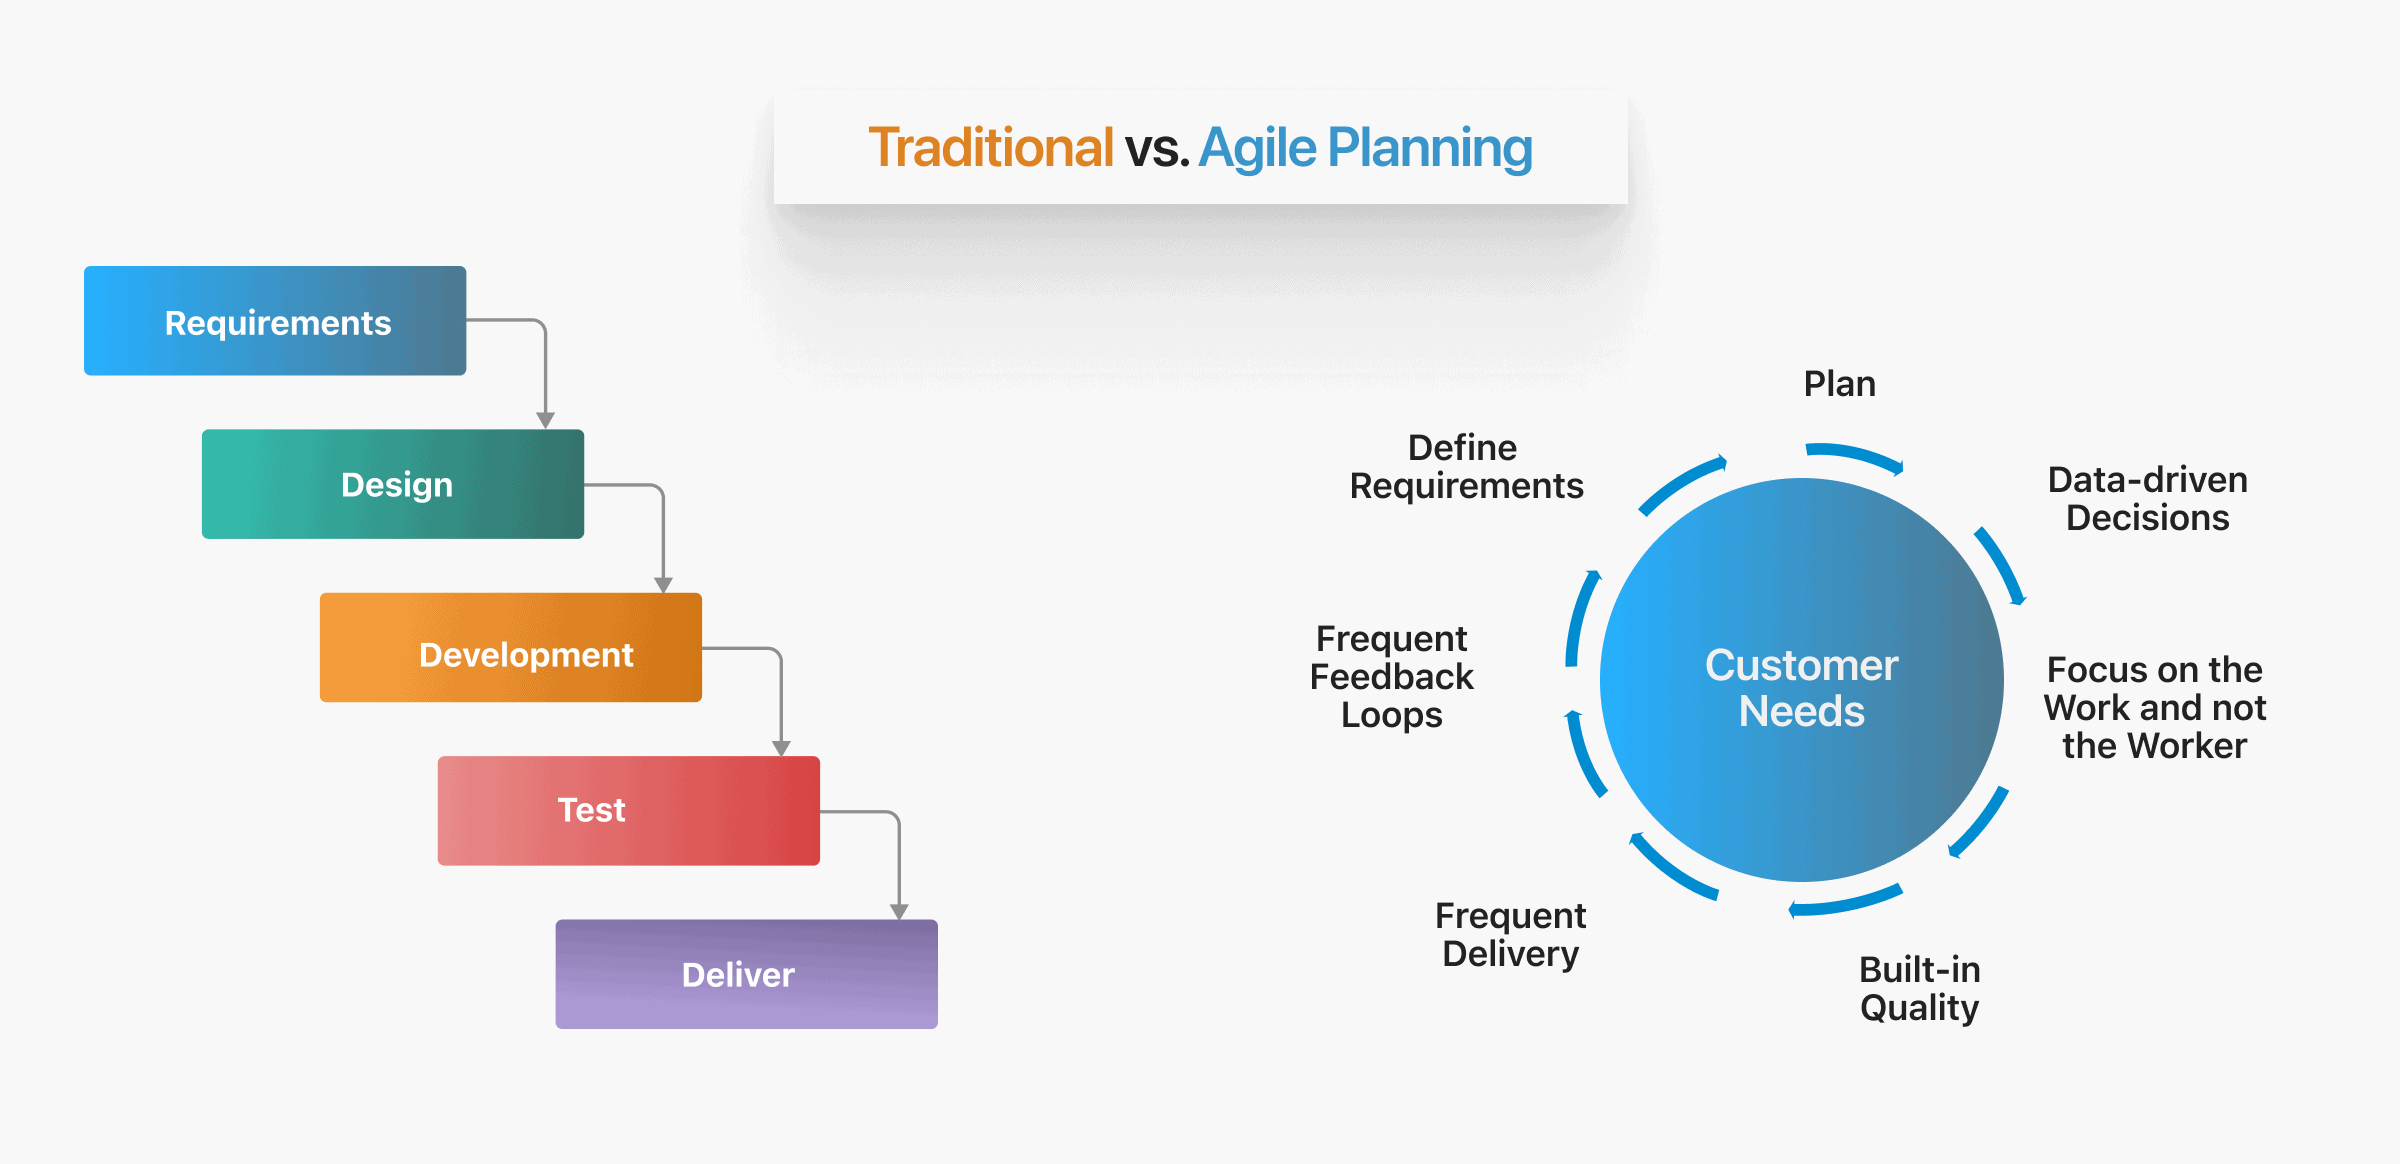
\includegraphics[width=0.9\textwidth]{Chapitres/Figures/agile.png}
    \caption{Agile vs approches classiques}
    \label{fig:agile}
\end{figure}

Parmi les méthodes agiles les plus reconnues dans le domaine du génie logiciel, on trouve 
Scrum, Kanban, Extreme Programming (XP), SAFe et Crystal. En vue de mener notre projet 
de manière efficace et de fournir un produit de qualité dans les délais impartis, nous 
avons opté pour la méthodologie \textbf{Scrum}.

%%%%%%%%%%%%%%%%%%%%%%%%%%%%%%%%%%%%%%%%%%%%%%%%%%%%%%%%%%%%%%%%%%%%%%%%%%
\subsection{La méthodologie Scrum}
%%%%%%%%%%%%%%%%%%%%%%%%%%%%%%%%%%%%%%%%%%%%%%%%%%%%%%%%%%%%%%%%%%%%%%%%%%

 \textit{"SCRUM est un cadre de travail dans lequel les personnes peuvent aborder des problèmes complexes et adaptatifs tout en livrant de manière efficace et créative des produits de la plus grande valeur possible.''} \cite{scrum}


Il s'agit d'une approche itérative et progressive qui évite l'effet \og tunnel \fg{}, où 
les résultats ne sont visibles qu'à la clôture du projet. C'est également une approche 
collaborative dans laquelle tous les membres de l'équipe sont actifs et contribuent aux 
décisions. Scrum s'articule autour de trois acteurs principaux :

\begin{itemize}[noitemsep, topsep=0pt]
    \item \textbf{Product Owner :} Il détient la responsabilité du produit ; c'est le client 
    qui communique ses attentes et approuve le travail lors des revues de sprint.
    \item \textbf{Scrum Master :} Il supervise le bon déroulement de la mission et résout 
    les obstacles qui entravent l'avancement du projet.
    \item \textbf{Scrum Team :} Ensemble d'individus en charge d'exécuter les exigences, 
    incluant développeurs, concepteurs et testeurs.
\end{itemize}

\begin{figure}[H]
    \centering
    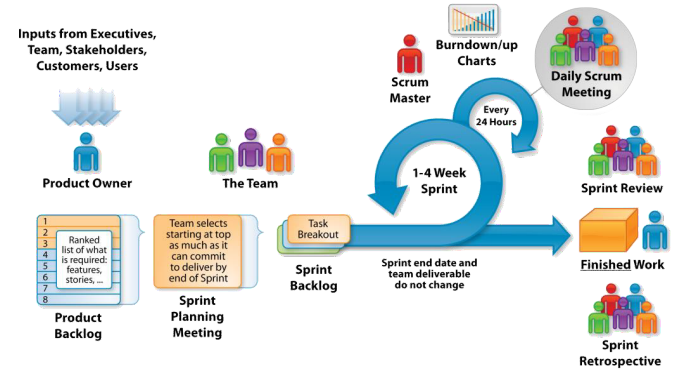
\includegraphics[width=0.7\textwidth]{Chapitres/Figures/scrum_model.png}
    \caption{Les caractéristiques du modèle Scrum}
    \label{fig:scrum_model}
\end{figure}

%%%%%%%%%%%%%%%%%%%%%%%%%%%%%%%%%%%%%%%%%%%%%%%%%%%%%%%%%%%%%%%%%%%%%%%%%%
\subsection{Product Backlog et Sprint Backlog}
%%%%%%%%%%%%%%%%%%%%%%%%%%%%%%%%%%%%%%%%%%%%%%%%%%%%%%%%%%%%%%%%%%%%%%%%%%

Dans la méthodologie Scrum, deux artefacts essentiels structurent la gestion des tâches 
et des priorités tout au long du projet.

Le \textbf{Product Backlog} est une liste ordonnée et exhaustive de toutes les 
fonctionnalités, exigences et améliorations souhaitées pour le produit final. Il est 
géré et priorisé par le Product Owner selon la valeur métier de chaque élément. Il 
évolue continuellement tout au long du projet en fonction des retours des parties prenantes 
et des besoins émergents. Chaque élément du Product Backlog est exprimé sous forme de 
\textbf{User Stories}, décrivant une fonctionnalité du point de vue de l'utilisateur.

Le \textbf{Sprint Backlog}, quant à lui, représente la sélection des User Stories issues 
du Product Backlog que l'équipe s'engage à réaliser durant un sprint donné. Contrairement 
au Product Backlog qui couvre l'ensemble du projet, le Sprint Backlog est limité à une 
itération précise (2 à 4 semaines) et appartient à l'équipe de développement. Il est 
défini lors du Sprint Planning et ne doit pas être modifié en cours de sprint.

\begin{table}[H]
\centering
\caption{Différence entre Product Backlog et Sprint Backlog}
\label{tab:backlogs}
\begin{tabular}{|p{3.5cm}|p{5cm}|p{5cm}|}
\hline
\textbf{Critère} & \textbf{Product Backlog} & \textbf{Sprint Backlog} \\
\hline
Portée & Ensemble du projet & Un seul sprint \\
\hline
Propriétaire & Product Owner & Équipe de développement \\
\hline
Contenu & Toutes les User Stories & User Stories sélectionnées \\
\hline
Évolution & Continu et dynamique & Figé pendant le sprint \\
\hline
Priorité & Définie par valeur métier & Définie par le Sprint Planning \\
\hline
\end{tabular}
\end{table}

%%%%%%%%%%%%%%%%%%%%%%%%%%%%%%%%%%%%%%%%%%%%%%%%%%%%%%%%%%%%%%%%%%%%%%%%%%
\section{Langage de Modélisation : UML}
\label{sec:uml}
%%%%%%%%%%%%%%%%%%%%%%%%%%%%%%%%%%%%%%%%%%%%%%%%%%%%%%%%%%%%%%%%%%%%%%%%%%

Pour la conception de notre système, nous avons adopté l'\textbf{UML} (Unified Modeling 
Language), un langage graphique composé de diagrammes offrant différentes 
perspectives sur le système en cours de réalisation.

\begin{figure}[H]
    \centering
    
\includegraphics[width=0.2\textwidth]{Chapitres/Figures/UML-logo.png}
    \caption{Logo UML}
    \label{fig:uml_logo}
\end{figure}

L'UML est un standard reconnu internationalement qui présente plusieurs atouts : il est 
sans ambiguïtés, universel, adaptable à tout langage orienté objet, et facilite la 
communication entre les membres de l'équipe et les parties prenantes. Dans le cadre de 
notre projet, nous utiliserons principalement le \textbf{diagramme de cas d'utilisation} 
pour modéliser les interactions entre les acteurs et le système, ainsi que le 
\textbf{diagramme de séquence} pour décrire le déroulement des scénarios fonctionnels.\cite{uml}

%%%%%%%%%%%%%%%%%%%%%%%%%%%%%%%%%%%%%%%%%%%%%%%%%%%%%%%%%%%%%%%%%%%%%%%%%%
\section{Conclusion}
%%%%%%%%%%%%%%%%%%%%%%%%%%%%%%%%%%%%%%%%%%%%%%%%%%%%%%%%%%%%%%%%%%%%%%%%%%

Dans ce premier chapitre, nous avons présenté notre organisme d'accueil Yes Internet ainsi que le cadre général du projet. Nous avons analysé les solutions existantes au niveau national et international, résumé leurs lacunes, et proposé notre solution adaptée au contexte tunisien. 

\medskip

Enfin, nous avons présenté la méthodologie de gestion de projet utilisée ainsi que le langage de modélisation qui guideront la conduite du projet.

\medskip

Dans le chapitre qui suit, nous aborderons la planification de notre projet.